\documentclass{article}
\usepackage[paperwidth=7.2in,paperheight=3.1in,margin=0.08in]{geometry}
\usepackage{tikz}
\usepackage{xcolor}
\usepackage{times}
\pagestyle{empty}

\definecolor{blue300}{HTML}{9FD2F5}
\definecolor{cardblue}{HTML}{2D5F9A}
\definecolor{attrgreen}{HTML}{2F855A}
\definecolor{edgegray}{HTML}{5A6470}
\definecolor{softgray}{HTML}{F3F5F7}

\usetikzlibrary{arrows.meta,positioning,shapes.geometric}

\tikzset{
  cardnode/.style={
    rectangle, rounded corners=5pt, draw=cardblue, very thick,
    fill=blue300!45, align=center, text width=1.35in,
    minimum height=0.52in, font=\bfseries\small
  },
  attrnode/.style={
    rectangle, rounded corners=4pt, draw=attrgreen, thick,
    fill=attrgreen!10, align=center, text width=1.12in,
    minimum height=0.34in, font=\scriptsize
  },
  edgelabel/.style={font=\tiny, fill=white, inner sep=1pt, text=edgegray},
  arrow/.style={-Latex, thick, draw=edgegray}
}

\begin{document}

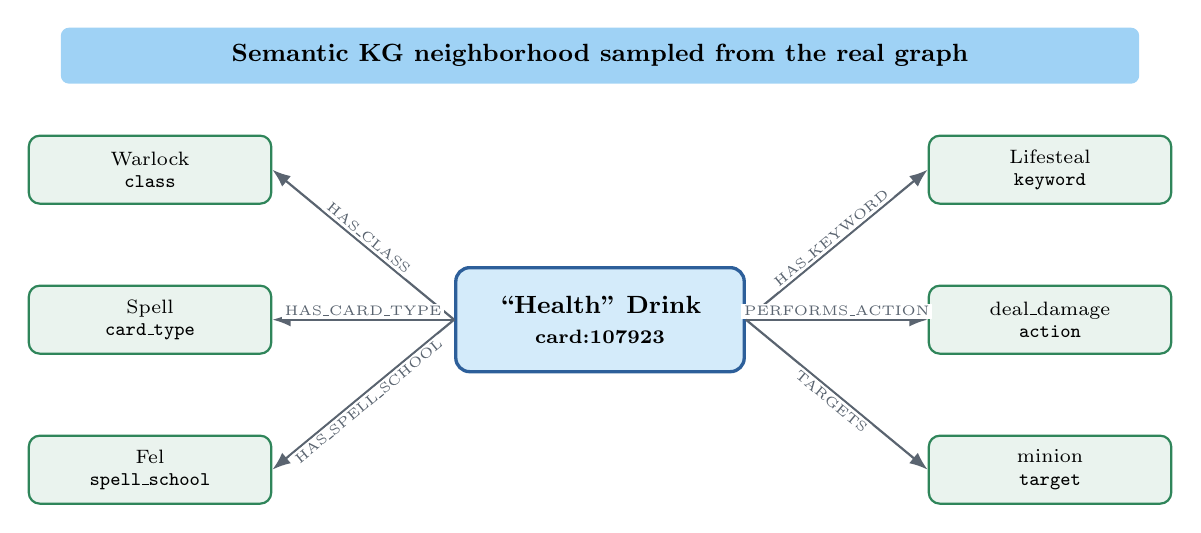
\begin{tikzpicture}[x=1in,y=1in]

  % Title
  \node[
    fill=blue300,
    rounded corners=3pt,
    text width=5.3in,
    minimum height=0.28in,
    align=center,
    font=\bfseries\small
  ] at (3.6,2.82)
  {Semantic KG neighborhood sampled from the real graph};

  % Center card
  \node[cardnode] (card) at (3.6,1.50)
  {``Health'' Drink\\ \scriptsize card:107923};

  % Left-side attributes, vertically aligned
  \node[attrnode] (warlock) at (1.35,2.25)
  {Warlock\\ \texttt{class}};

  \node[attrnode] (spell) at (1.35,1.50)
  {Spell\\ \texttt{card\_type}};

  \node[attrnode] (fel) at (1.35,0.75)
  {Fel\\ \texttt{spell\_school}};

  % Right-side attributes, vertically aligned
  \node[attrnode] (lifesteal) at (5.85,2.25)
  {Lifesteal\\ \texttt{keyword}};

  \node[attrnode] (damage) at (5.85,1.50)
  {deal\_damage\\ \texttt{action}};

  \node[attrnode] (minion) at (5.85,0.75)
  {minion\\ \texttt{target}};

  % Edges
  \draw[arrow] (card.west) -- node[edgelabel, above, sloped] {HAS\_CLASS} (warlock.east);
  \draw[arrow] (card.west) -- node[edgelabel, above] {HAS\_CARD\_TYPE} (spell.east);
  \draw[arrow] (card.west) -- node[edgelabel, below, sloped] {HAS\_SPELL\_SCHOOL} (fel.east);

  \draw[arrow] (card.east) -- node[edgelabel, above, sloped] {HAS\_KEYWORD} (lifesteal.west);
  \draw[arrow] (card.east) -- node[edgelabel, above] {PERFORMS\_ACTION} (damage.west);
  \draw[arrow] (card.east) -- node[edgelabel, below, sloped] {TARGETS} (minion.west);

\end{tikzpicture}

\end{document}